\documentclass{article}
\usepackage[utf8]{inputenc}
\usepackage{amsmath}
\usepackage{amsfonts}
\usepackage{stmaryrd} % more math symbols
\usepackage{amsthm} % for theoreme style


%%%% for images
\usepackage{graphicx}
\graphicspath{ {./rapports} }

%%%% to set boxes like a theorem
\theoremstyle{definition}
\newtheorem{definition}{Definition}[section]

\theoremstyle{property}
\newtheorem{property}{Property}[section]

\theoremstyle{remark}
\newtheorem*{remark}{Remark}
%%%% to insert a line of code in the text with \texttt{ code }
\newcommand{\code}[1]{\texttt{#1}}


\title{Project Report v1}
\date{June 2022}

\begin{document}
	\section{Introduction}
	Tsunamis do not occur very often but are devastating phenomena. Research and studies about tsunamis try to predict the impact of such events to protect people.
	Due to the sheer scale of tsunami, laboratory and analytical models are not relevant. The former because we can not obtain an equivalent scale model in a lab, the latter because there is no analytical solution to the propagation equations.
	Although a numerical resolution can approximate the solution, it requires a huge computing power and time without taking into account the accuracy errors due to turbulence phenomena.\\


	But then, how could we speed up fluid mechanics calculations?

	\section{Neural Networks}
	Now the basis of multiple state of the art technologies in data science, neural networks provide a framework we hope can solve propagation equations in a shorter time than with regular finite elements.\\
	For now, we will focus on the study of multilayer perceptron, one of the first neural networks to have been developped. They consist in an input layer, a vector of $n$ components, and an output layer, of $p$ components.
	The input is subjected to a series of linear operations and non-linear activations are applied trough "hidden layers" to get the output.\\
	A multilayer perceptron can then be seen as a non linear function:
	$$ \mathcal{N} : \mathbb{K}^n \rightarrow \mathbb{K}^p $$

	If we note $g_i$ the (non-linear) activation function, and $W_i$ and $b_i$ the weight and bias matrix of the ith hidden layer, then, for a MP with k hidden layers:
	$$ \forall x \in \mathbb{K}^n, \mathcal{N}(x) = g_k(b_k + W_k g_{k-1}(b_{k-1}+W_{k-1} g_{k-2}(\dots(b_1 + W_1 x)))) $$
	Through training epoch, passes through the training dataset coupled with gradient descent, we want $\mathcal{N}$ to approach a function of interest.

	\section{Partial Differential Equation}
	Our goal is to solve the propagation equation of a tsunami, which is a partial differential equation (PDE). In a general sense, a PDE is defined as:
	\begin{equation*}
		(E): 
		\begin{cases}
			\mathcal{Q}(u, \nabla u, H u, \dots)(x) = 0 & \text{inside $\Omega$}\\
			\mathcal{R}(u, \nabla u, H u, \dots)(x) = f(x) & \text{on $\partial \Omega$}
		\end{cases}
	\end{equation*}

	Where $\mathcal{Q}$ and $\mathcal{R}$ are linear operators, $\Omega$ is the domain considered,\\
	and $u : \mathbb{K}^n \rightarrow \mathbb{K}^p$ is the solution to $(E)$.\\
	
	Our goal is to replace $u$ with a neural network $\mathcal{N}$ and train it to get a solution to $(E)$.
	However, this would mean training on both the domain and its boundary. To avoid this case as the boundary is always defined with boundary conditions, we reformulate the problem:\\

	Instead we replace $u$ with $\Psi$ defined as:
	$$\Psi(x) = A(x) + F(x)*\mathcal{N}(X)$$
	Where $A$ verifies the boundary conditions, and $F$ is null on the boundary.\\
	As such, we unconstrained the problem, and the neural network can train inside the domain, with the boundary conditions handled by the above mentionned functions.

	\section{Find A}
	In this section we propose two choices for the function $A$ in 2 different contexts.\\
	Let $K$ be a point in space with coordinates 
	\begin{math}
	\Vec{x_K} = \sum x_j\Vec{e_j}
	\end{math}

	\subsection{Function 1}
	\begin{equation*}
		\forall x \in \mathbb{R}^k, \psi_K(x)=
		\left\{
		\begin{matrix}
		\exp \left( -\frac{1}{l^2 - d(x,K)^2} \right) & if \ d(x,K)^2<l^2\\
		0 & else
		\end{matrix}
		\right\}
	\end{equation*}
	Where 
	\begin{math}
	d(x,K)^2 = \lVert x - x_K \rVert^2
	\end{math}
	\\
	This function has the advantage of not interacting with the space located beyond a distance $l$ away from point $A$

	\subsubsection{Use in our case}
	Let $\Omega$ be a domain, and $\partial\Omega$ its boundary. We sample $N$ points from the boundary with coordinates $x_i$ such as $g(x_i)=g_i$. Let us use 
	\[
	l = \min_{1\leq i,j \leq N}\lVert x_i - x_j \rVert
	\]
	\\
	Then, we can use the following function to compute the value of the boundary with interesting properties.
	\begin{equation*}
		\Psi(x) = \exp \left( \frac{1}{l^2} \right) \sum_{i=1}^{N}g_i\psi_i(x)
	\end{equation*}

	\subsubsection{Boundary conditions} 
	We do verify the boundary conditions :
	\begin{equation*}
		If \ x=x_j\in \partial \Omega, \Psi(x_j) = g_j
	\end{equation*}

	As by hypothesis, for $\psi_j$ the distance is null, and for all other $\psi_i$ we are at a distance greater than $l$ away from $x_i$.

	\subsubsection{Regularity}
	By summing $\psi$ functions, we have that $\Psi$ is a class $C^\infty$ function.

	\subsubsection{Derivative}
	By using chain rule, we can easily calculate the derivative according to any variable j with
	\begin{equation*}
		\partial_j \Psi(x) = \exp\left(\frac{1}{l^2}\right)\sum_{i=1}^{N}g_i\partial_j\psi_i(x)
	\end{equation*}
	and
	\begin{equation*}
		\partial_j\psi_i(x) = \frac{-2(x_j-x_{Aj})}{(l^2 - d(x,i)^2)^2}\psi_i(x)
	\end{equation*}

	\subsubsection{Bounded function}
	By definition, we have
	\begin{equation*}
		\forall x \in \mathbb{R}^k, \min_{1 \leq i \leq N}g_i \leq \Psi(x) \leq \max_{1 \leq i \leq N}g_i
	\end{equation*}

	\subsubsection{Ease of computation}
	To calculate $\Psi$ and its gradient, a lot of elements are redundant and thus can be evualated once, like $l$ (when we sample the boundary) and $l^2-d(x,i)^2$ for each point of the boundary.

	\subsubsection{Issues}
	This function is too restrictive to be usable in practice. With too much sample boundary points, this function becomes a series of spikes, and thus does not approximate the boundary asymptotically.\\
	In case of a small amount of samples, this function is useful.

	\subsection{Function 2}
	\begin{equation*}
		\forall x \in \mathbb{R}^k, \psi_K(x)= 1 - \tanh \left( \frac{d(x,K)}{l} \right)^2
	\end{equation*}

	This time with:
	\begin{equation*}
		\Psi(x) = 0.5 \sum_{i=1}^{N}g_i\psi_i(x)
	\end{equation*}

	This time, our function verifies the boundary conditions only asymptotically with a uniformly sampled boundary.\\
	The $0.5$ coefficient is their to correct for the first order interactions between two adjacent $\psi_K$.\\
	Through numerical simulations, we obtain a smoothed boundary that closely ressembles the real boundary with enough sample points.
	In our simulation, this function will be mostly used as the $A$ function.

	\section{Find F}
	Set $(d,n)\in \mathbb{N}^*$ and $(x_i)_{i\in \llbracket0;n-1\rrbracket }\in \mathbb{R}^{d}$ distinct one another. We seek a polynomial $F\in\mathbb{K}[X]$ such that $\mathbb{K} \in \{\mathbb{R},\mathbb{C}\}$ and
	$$\forall i\in \llbracket1;n\rrbracket,~F(x_i)=0 \text{ and } \exists x_n:~F(x_n)\neq0$$
	
	\subsection{Case 1D}
	In the case $d=1$, Vandermonde polynomials are a good start. The only thing to add to the construction is a point where the polynomial $F$ is not null. Assuming the orthobarycentre of the family $(x_i)_{i\in \llbracket0;n-1\rrbracket }$ is not already inside, let's take the orthobarycentre of these points defined as $x_n:=\frac{1}{n}\sum_{i=0}^{n-1} x_i$.\\
	The system induced is this one :
	\begin{equation*}
		\begin{pmatrix}
			1 & x_0 & \dots & x_{0}^{n} \\
			\vdots & \vdots & \ddots & \vdots\\
			1 & x_{n-1} & \dots & x_{n-1}^{n} \\
			1 & x_n & \dots & x_n^{n-1} 
		\end{pmatrix}
		\begin{pmatrix}
			a_0\\
			\vdots\\
			a_{n-1}\\
			a_{n}
		\end{pmatrix}
		=
		\begin{pmatrix}
			0\\
			\vdots\\
			0\\
			1
		\end{pmatrix}
	\end{equation*}
	that one can solve thanks to the inversion of the Vandermonde matrix, which is non-singular since all the points are distinct one another thanks to the assumption.
	
	
	\subsection{Case 2D}
	The work done here for $d=2$ is meant to be easily generalizable to even greater values of $d$.
	Set $\forall i \in \llbracket0;n-1\rrbracket, x_i \text{ has as coordinates }(x_{i,0},x_{i,1})$.
	
	\subsubsection{Matrix method}
	\subsubsection*{Start of an idea (inspired from Vandermonde matrix in 1D)}
	Globally, $F$ can be defined in $\mathbb{R}_{n+1}[X]$ considering its roots $(x_i)_{i\in \llbracket0;n-1\rrbracket }$ and the point $x_n$ where it is not null. Therefore, set $x_n$ the orthobarycentre with the same assumption as previously 	and $(\alpha_{ij})_{\{(i,j)\in\mathbb{N}:i+j\leq n\}}\in\mathbb{R}^{2n}$ such that
	\begin{equation*}
		\forall (x,y) \in \mathbb{R}^2,~F(x) = \sum_{\{(i,j)\in\mathbb{N}:i+j\leq n\}} \alpha_{ij}x^iy^j
	\end{equation*}
	\begin{equation*}
		\begin{pmatrix}
			1 & x_{0,0} & x_{0,1} & x_{0,0}x_{0,1} & \dots & x_{0,1}^{n} \\
			\vdots & \vdots&\vdots & \vdots& \ddots & \vdots \\
			1 & x_{n-1,0} & x_{n-1,1} & x_{n-1,0}x_{n-1,1} & \dots &x_{n-1,1}^{n} \\
			1 & x_{n,0} & x_{n,1} & x_{n,0}x_{n,1} & \dots & x_{n,1}^{n} \\
		\end{pmatrix}
		\begin{pmatrix}
			\alpha_{00}\\
			\vdots\\
			\alpha_{0(n-1)}\\
			\alpha_{0n}
		\end{pmatrix}
		=
		\begin{pmatrix}
			0\\
			\vdots\\
			0\\
			1
		\end{pmatrix}
	\end{equation*}

	Actually, Vandermonde does not give any proof of the non-singularity of the left matrix and one could thought about putting more combinations of the coordinates of each point to extract a non-singular matrix after.
	Yet, finding this extracted matrix remains computationally heavy in addition to being uncertain.\\
	
	\subsubsection*{In hindsight}
	The realm this idea steps into is the realm of principal component analysis. It remains interesting considering the fast differentiation of the polynomial one could get after. Nevertheless, it could force us to already use machine learning which will require some time to compute accurately and will always remain an approximation of the true solution we seek.

	
	\subsubsection{Direct approach}
	In this kind of situation, constructing the polynomial $$F:(x,y)\mapsto\prod_{m=0}^{n-1}(x-x_i)(y-y_i)$$ quickly comes to mind. Nevertheless, $F$ would be to often null on the domain and could induce great errors after. So, the idea is to replace the given factor by one null only at a given point as shown here:
	\begin{definition}\label{F_real}
		$$\forall (x,y)\in\mathbb{R}^2,~F_r(x,y) = \prod_{k=0}^{n-1}((x-x_k)^2 + (y-y_k)^2)$$
	\end{definition}
	
	\begin{definition}\label{F_comp}
		$$\forall (x,y)\in\mathbb{R}^2,~F_c(x,y) = \prod_{k=0}^{n-1}((x-x_k) + i(y-y_k))$$
	\end{definition}
	
	\begin{remark}[comparison]\
		\begin{itemize}
			\item $\forall (x,y)\in\mathbb{R}^2,~F_r(x,y)=\vert F_c(x,y) \vert^2$
			\item the coefficients of $F_c$ are faster to compute but harder to evaluate than the ones of $F_r$
		\end{itemize}
		
	\end{remark}
	
	\newpage
	\section{Hyperparameters}
	Here is the scheme of model tuning followed:
	\begin{figure}[h]
		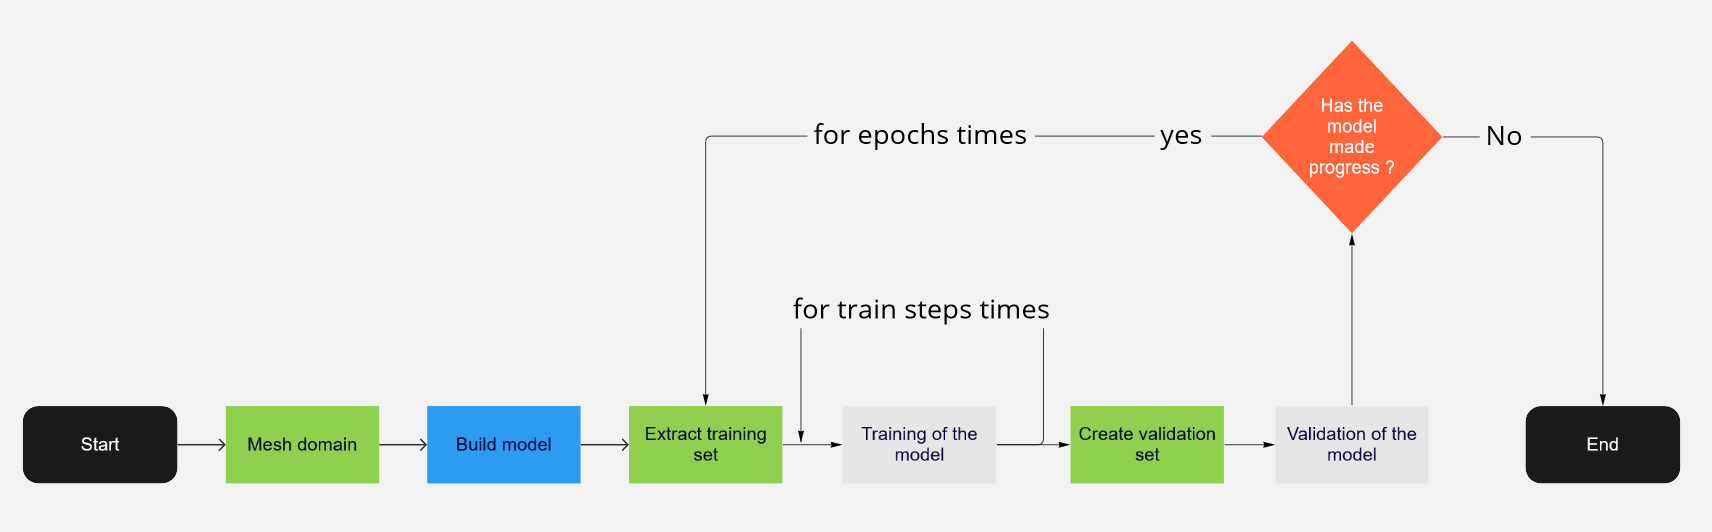
\includegraphics[width=13cm, height=4cm]{tuning_model.png}
		\centering
		\caption{scheme of a model tuning}
	\end{figure}
	\begin{remark}
		The red box involves using an early stopping callback to stop the epoch loop when the model begins to overfit. A \texttt{patience} integer set how far the system will go back in history. If during \texttt{patience} epochs the has not made progress the epoch loop is stopped.
	\end{remark}
	
	The hypertuning comes when one wants to construct a model and a training that will end to a low validation error. Let's list all the hyperparameters involved in this scheme applied for the Poisson equation on a square domain:
	\begin{itemize}
		\item \texttt{grid\_length}: integer setting the number of points in the domain to \texttt{grid\_length}x\texttt{grid\_length}
		\item \texttt{l\_units}: list of integers depicting the number of hidden layers and the number of neurons per layer of the sequential machine learning model
		\item \texttt{l\_activations}: list depicting the activation functions of each layer of the model
		\item \texttt{noise}: integer in $\{0,1\}$ conditioning the use of a Gaussian layer of mean $0$ after the input layer
		\item \texttt{stddev}: the standard deviation of the Gaussian layer when it is used
		\item \texttt{optimizer}: string depicting the optimizer used
		\item \texttt{learning\_rate}: float setting the learning rate of the previous optimizer
		\item \texttt{epochs\_max}: integer setting the number of maximum epoch loops
		\item \texttt{n\_trains}: integer setting the number of train loops
		\item \texttt{batch\_size}: integer setting the number of points extracted from the mesh to construct the training set at each epoch loop
		\item \texttt{patience}: integer setting how many epoch loops the system can go on without progressing, after that the trial is ended
	\end{itemize}
	
	An automatization of the hypertuning by hand and using Keras Tuner has already been led. Nevertheless, some work must still be done to assure a low validation error with minimal cost of time and hardware. A few bugs, impeding a proper convergence, also seems to persist in some of our implementations.
	
	
	
\end{document}
